\section{Versuchsaufbau und Justierung}

Der Versuchsaufbau besteht aus einem Szintillator-Tank mit einem ungefähren Volumen von 50 Litern. An jedem Ende des Tanks sind Photomultiplier (PM) montiert, die die durch Myonen oder deren Zerfallsprodukte verursachten Szintillationssignale detektieren. Eine Kombination von NIM-Modulen ermöglicht die Messung des Zeitintervalls zwischen den gleichzeitig eintreffenden Myon- und Zerfallsproduktsignalen. Die Ausgänge der beiden PMs werden über eine Verzögerung zu einem Diskriminator mit einstellbarer Schwelle geführt. Auch die Dauer des Ausgangsimpulses des Diskriminators ist einstellbar. Beide Signale gelangen dann in eine Koinzidenzschaltung, die nur ein Ausgangssignal erzeugt, wenn die Eingangsimpulse gleichzeitig eintreffen. Dies wird von der elektronischen Entsprechung einer Stoppuhr gefolgt.

Das Ausgangssignal der Koinzidenzeinheit erreicht zwei UND-Gatter und über eine weitere Verzögerungsleitung von $\symup{\Delta} t = 30 \, \text{ns}$ ein Monoflop. Dieses setzt die Suchzeit $T_s$ als Abstand zwischen initialem Umschalten, wenn das Signal ankommt, bis zum Zurückschalten in den Ausgangszustand. Die UND-Gatter sind mit dem Zeit-Amplituden-Umsetzer (TAC) so verbunden, dass eines die Zeitmessung startet, während das andere sie stoppt. Zwei Zähler zählen jeweils die Start- und Stoppimpulse. Eine geeignete Kombination von Komponenten stellt sicher, dass die Zeitmessung startet, wenn ein Myon in das aktive Volumen eintritt. Zerfällt das Myon im Tank, wird die Messung gestoppt.

Das Signal vom TAC gelangt in den Mehrkanalanalysator (MCA), der von einem PC gesteuert wird. Zur Kalibrierung des MCA steht ein Doppelpulsgenerator (DPG) zur Verfügung, der zwei Pulse mit variablem Zeitintervall bei einer Frequenz von 1 kHz erzeugt.
Wenn die PMs mit Hochspannung versorgt werden, sollten an den jeweiligen Ausgängen Spannungspulse mit variierenden Amplituden sichtbar sein. Dies wird mit Hilfe eines Oszilloskops überprüft.

\enlargethispage{\baselineskip}

Im nächsten Schritt wird die Schwellenwertspannung der Diskriminatoren so eingestellt, dass an beiden Ausgängen etwa 30 Pulse pro Sekunde gemessen werden. Eine Impulsdauer von $\symup{\Delta} t = 10 \, \mu\text{s}$ wird eingestellt. Dazu wird der Pulszähler angeschlossen. Um die Koinzidenzapparatur anzupassen, wird systematisch eine der Verzögerungsleitungen variiert und die Pulsrate am Ausgang der Koinzidenzeinheit beobachtet. Der Messbereich sollte groß genug sein, um die Halbwertsbreite der Verteilung zu bestimmen. Schließlich wird eine geeignete Verzögerung für die gesamte Messung gewählt. Die Ereignisrate sollte etwa $20 \, \text{s}^{-1}$ betragen.

\begin{figure}[H]
    \centering
    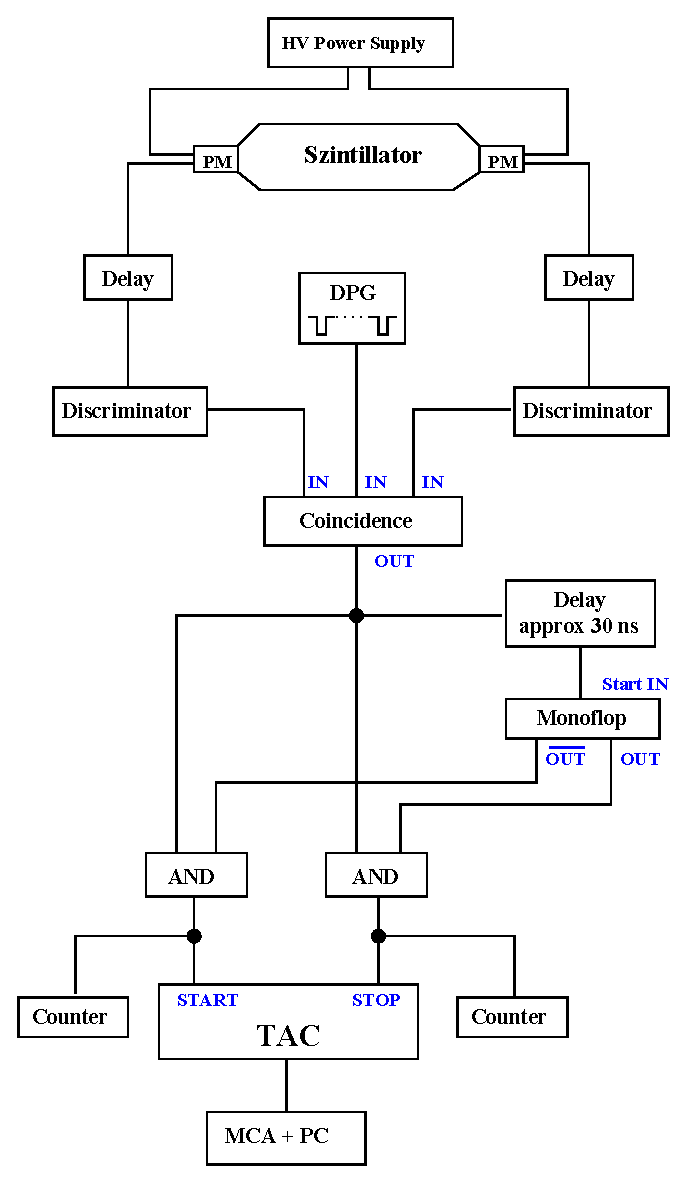
\includegraphics[width=0.55\textwidth]{content/grafik/Aufbau.pdf}
    \caption{Schematische Darstellung des verwendeten Versuchsaufbaus \cite{myon}.}
    \label{fig:Aufbau}
\end{figure}

Die restlichen Teile der Schaltung werden angeschlossen. Eine Suchzeit $T_s$ wird am Monoflop eingestellt und der Messbereich des TAC entsprechend angepasst.

Zur Kalibrierung des MCA wird der Doppelpulsgenerator angeschlossen und gemessen, welches Zeitintervall der Doppelpulse welchem Kanal des MCA entspricht. Um eine gleichmäßige Effizienz über den gesamten Messbereich zu überprüfen, wird für alle Messpunkte die gleiche Messzeit gewählt und die absoluten Zählraten verglichen.

Nach erfolgreicher Kalibration wird die Messung der Lebensdauer der Myonen gestartet.

\section{Messung}

Die in \autoref{fig:Aufbau} gezeigte Schaltung wird eingerichtet und die Lebensdauer der kosmischen Myonen aus einer Reihe von Messungen der einzelnen Lebensdauern bestimmt.
